\documentclass{llncs}

%% Verwende A4-Format statt Letter
\usepackage{a4}
%% Deutsche Silbentrennung und Sprache (neue Rechtschreibung)
%\usepackage[ngerman]{babel}
%% Verwende Schriftart mit "echten" Umlauten statt Akzenten
\usepackage[T1]{fontenc}
%% Verwende Umlaute direkt
\usepackage[utf8x]{inputenc}
%% Hyperlinks für interne Referenzen
\usepackage{hyperref}
%% Grafiken einbinden
\usepackage{graphicx}
%% Paket für Unterabbildungen pro Abbildung
%\usepackage{subfig}
\usepackage{todonotes}

% Titel der Arbeit
\title{Peer-To-Peer in Botnets}

% Angaben zum Author
\author{Moritz Marc Beller}
\institute{%
   Fakultät für Informatik, \\
   Technische Universität München \\
%    Munich, Germany\\
   \email{\{beller\}@in.tum.de}
}

\pagestyle{plain}

%------------------------------------------------------------------------------
\begin{document}

\maketitle

%------------------------------------------------------------------------------
\begin{abstract}
In this literature review paper, we describe a relatively novel means
of communication in botnets, namely {\it peer-to-peer} (P2P)
communication.  While many users are familiar with P2P file sharing,
the term has attracted more attention lately as malicious botnets such
as Storm\cite{davis2008sybil} have emerged, causing quantifiable
real-world damage.

After we explain P2P botnets and compare them to conventional botnets,
we describe possible countermeasures against P2P botnets and give an
outlook into the future of these.

Having read this article, the reader will be well-informed about
current and future techniques in P2P botnets.
\end{abstract}

%------------------------------------------------------------------------------
\section{Introduction}

%\subsection{Motivation for Research on P2P botnets}
Cyber-attacks are a growing threat to the security of the world. As a
result, in June of 2011, the German government founded a ``national
defence centre against cyber crime''.\cite{cyber} This step became
necessary as new forms of computer worms are no longer restricted to
harming only computers and the data stored on them, as the example of
``Stuxnet'' demonstrates:

 In 2010, a new computer worm called ``Stuxnet'' was discovered. It is
 suspected to have damaged Iran's uranium centrifuges, giving it the
 title ``the first cyber weapon''\cite{benzin2011first}. To spread and
 update, Stuxnet used Internet and Intranet structures to build its
 own {\it botnet}.\cite{fallierew32} Although Stuxnet didn't try to
 build an armada of infected computers like most other bots do,
 Stuxnet is in alignment with a series of new botnets using {\it
   peer-to-peer} communication instead of a centralised server.

This review paper focuses on these peer-to-peer botnets and the
growing threat emerging from them. 

\subsection*{Outline}
We start by introducing common botnet terminology. We then give a
classification of P2P botnets and distinguish different architectures
of botnets. In the following sections, we describe the typical
lifetime of a P2P botnet, the command and control structure in P2P
botnets, comparing conventional botnets to P2P botnets. In the
remainder of this review paper we described possible countermeasures
against P2P botnets and draw conclusion on what types of botnets to
expect in the future.


\section{Definitions}
A computer able of executing commands remotely triggered by a
malicious attacker and possibly against the will of the owner is
called a {\it bot} or {\it zombie.} The term can also generally refer
to the program executed, meaning not a special instance of an infested
computer, but the software or idea behind the software per se (as in
``the Storm bot'').

A {\it botnet} is a group of bots forming a common network
structure.\cite{schoof2007detecting} In most recent papers on the
subject (\cite{wang2009systematic}, \cite{abu2006multifaceted}), the
term botnet is defined as purely negative, i.e. a network performing
destructive aims such as denial-of-service
attacks\footnote{Abbreviated: DoS attacks, i.e. generating so much
  traffic the target cannot function normally any more}, sending spam
or hosting a phishing website\cite{steggink2007detection}. Other
common aims include providing the aggregated CPU resources of the
botnet, stealing users' credentials \cite{borgaonkar2010analysis} or
doing click fraud.\footnote{Click fraud is the process of generating
  clicks on web banners without an actual user seeing or clicking the
  advertisement, for the sake of making money.} on affiliate
networks\cite{clickFraud}

In the following, we use a bias-free definition of botnet as per
our understanding technology is generally ethics-free. Additionally,
there are many examples where botnets are used in a non-destructive
way (e.g. \cite{seti}), or even to destroy existing malicious botnets.

The controller of the botnet is referred to as the {\it
  botmaster}. He doesn't necessarily have to be the founder of the
botnet (cf. section \ref{ClassificP2P}).

The expression {\it bot candidates} specifies the set of computers
which are target to becoming a bot themselves.

{\it P2P}, short for {\it Peer-to-Peer}, being a technology buzz word
of the internet in the late 1990s with the upcoming file sharing
services like Napster\cite{napster}, has attracted less attention in
recent years. P2P defines an unstructured information network amongst
equals --- so-called peers. Two or more peers can spontaneously
exchange information without a central instance. According to
\cite{schoder2005core} ``P2P networks promise improved scalability,
lower cost of ownership, self-organised and decentralised coordination
of previously underused or limited resources, greater fault tolerance,
and better support for building ad hoc networks.''  These properties
coupled with the fact that files exchanged in P2P networks are prone
to malware, trojans and viruses make P2P networks a most-attractive
base for building botnets.  Well-known P2P networks include the
Napster, Gnutella, Overnet and Torrent network.  

A {\it P2P bot} then is a bot that uses a P2P protocol as a means of
communication with other bots.

The so-called {\it C\&C}, command and control structure, specifies
the way and protocols in which the botmaster and the bots communicate
with each other. It is the central property of any botnet. Common
protocols for C\&C include IRC, HTTP, FTP and
P2P.\cite{borgaonkar2010analysis}

{\it IRC} --- internet relay chat --- is a ``teleconferencing
system''\cite{irc}, typically used for text chatting in channels
joined by a large number of participants. While its protocol is
relatively easy to implement, it provides a lot of features. It has
thus become the one of the most widely-used protocols for C\&C in
conventional botnets.

The process of {\it bootstrapping} generally describes starting a more
complex system out of a simple system. In regard to botnets, the
term usually means loading of the bot code (often injected into the
original file sharing program) and establishing a connection to other
bots.\cite{wang2009systematic}


\section{An overview over P2P botnets}
This section shall give a short overview of P2P botnets: How they came
into being, how one can classify them according to their distribution
strategy and what the typical life of a botnet looks like.

\subsection{A brief history of botnets}
The origins for the term ``bot'' go back to so-called IRC bots, short
for IRC robots. An IRC bot is a program that handles specific tasks in
the IRC automatically, so that the administrator does not need to do
those routine jobs.

The first IRC bot ever to be created was named Eggdrop. Its origins go
back to the year 1993. However, in April 1998 a deviant called
GT-Bot appeared and formed the first malicious botnet, using IRC's
C\&C structures. Four years later, in 2002, Slapper was the first
botnet to make use of P2P for C\&C.\cite{li2009botnet}

There have been many more P2P botnets created since, most notably
perhaps the Phatbot and Storm botnets. Phatbot (also called Agobot,
Gaobot) became renowned for its large set of built-in attacks ranging
from password sniffing to DoS.\cite{cooke2005zombie} The storm botnet,
which exists in several different versions, was described ``as one of
the most sophisticated botnet[s] active
today''\cite{davis2008sybil}. Storm is based on the Overnet network, a
P2P network established by programs such as eMule and eDonkey.

 A criminal conviction because of launching a botnet is relatively
 seldom, since botmasters try to hide their identities (see ``stepping
 stones'' in figure \ref{central-network}). Yet, in 2007, John
 Schiefer was sentenced to four years in prison. He built a botnet
 with up to 250,000 zombies, collecting passwords and bank credentials
 from the bots.\cite{BotnetCrime}


\subsection{Classification of P2P networks}
\label{ClassificP2P}
There are three types of P2P networks: {\it parasite, leeching} and
{\it bot-only.}\cite{wang2009systematic} 

Parasite and leeching bots infiltrate existing P2P networks, while
``bot-only'' networks are designed with new network protocols. 

Parasite botnets recruit new bots only from the set of existing P2P
participants; they try to infect system inside the P2P network and
make them become bots. Due to the often illegal content distributed in
file sharing networks, they are a perfect culture medium for viruses,
malware and worms. It is thus convenient for an attacker to spread a
highly-demanded file (e.g. some cracked computer game, software or
porn) containing the injection code sequences for his bot. This code is
then injected into the file sharing client. Vulnerable hosts in the
network are infected this way. On the downside, this means that the
spread of the bot is limited to the size of the P2P network.

In contrast, leeching bots not only try to infiltrate systems which
are already part of the P2P network, but also systems outside of the
P2P network. Naturally, they are bigger in size as they have to
deliver the P2P client, too. This might be more difficult to achieve
as it means that systems must unwillingly take part in the
network. Often, firewalls and port-forwarding are not configured for
use with the P2P network on these systems, reducing the performance of
the botnet: Since the owner of the computer usually doesn't even know
he is participating in a P2P network, he has no intention of opening
the ports in his firewall. Leeching bots can spread through any
possible measure: File sharing, downloads on websites, email
attachments or instant messaging, to name a few.

There are good reasons for either strategy --- relying on existing
networks or creating a new one: Using an extant P2P network as a base
--- like parasite and leeching bots do --- unburdens the botmaster
from setting up and building a botnet infrastructure. It profits from
the established P2P network, making use of filtering, error-correction
and encryption as far as the chosen network has support for it. On the
other hand, features are limited to the existing P2P protocol. A
specifically-built P2P bot-only network is naturally more tailored
towards its purpose. Due to the bot-exclusive memberships, it might be
easier to shutdown the botnet for an attacker as all participants can
be considered bots and there is no risk of accidentally shutting down
an innocent member. Bot-only networks are described in detail in
section \ref{decent}.


\subsection{Lifetime of P2P botnets}
Wang et al.\cite{wang2009systematic} differentiate three stages of P2P botnets:
\begin{itemize}
\item Recruiting bot members (infecting others)
\item Forming the botnet (construction phase)
\item Standing by for instruction \\
This is the actual ``operational'' phase of the botnet. Bots are awaiting instructions from their master. Instructions can either be actual commands or performing updates. In this phase, the chosen C\&C structure is essential.
\end{itemize}
It should be noted that these phases are not strictly exclusive,
e.g. during the third phase (standing by for instruction), building of
the botnet may well continue. In fact, this is an inherent property of
any P2P network: Constant transformation of the network. It is only
until a critical mass of bots has proceeded past phase one and two,
that the botnet can be called operational.

When speaking about P2P networks, a factor that must be taken into
consideration is the {\it churn} of the network. By this name, we
describe the collective effects that the independent connects and
disconnects of thousands of peers can have. The term churn also refers
to the different session lengths (most P2P users typically have their
PC running for several hours, while there are some which stay
constantly online). In short, churn stands for the dynamics in a P2P
system. Despite its great significance, churn has not been discussed
in the literature a lot. \cite{stutzbach2006understanding}

\section{Command and Control structures in botnets}
In this section, we give an overview of the C\&C typically used in P2P
botnets and compare it to the C\&C in centralised architectures. The
differences in C\&C are the most notable differences between the two,
apart from the architecture itself (cf. section \ref{architecture}). There
exist three fundamentally different forms of C\&C in botnets:
Centralised C\&C, P2P C\&C and unstructured C\&C. After clarifying the
differences between push and pull communication, we explain the three
approaches.


\subsection{Push/Pull mechanism}
\label{pushpull}
Commands can be distributed in two ways: Either via a push or a pull
mechanism. ``Pulling'', being the more trivial of the two approaches,
is the process of a client actively asking a server whether there's
new instructions for it. To be up-to-date, this has to be performed
periodically, increasing network load.  Push on the other hand is
technically more advanced, as commands from the server will be
automatically ``forwarded'' to the clients --- the difference between
push and pull in a bot is much like IMAP IDLE compared to POP3 for
mail: With POP3, the user client has to periodically ask the server
whether there are new messages available (pull), whereas with IMAP,
the client gets a new message pushed by the server. This has the
advantage of reducing the network traffic, but it requires that the
server can open a connection to the clients (cf. section \ref{nat}).


\subsection{C\&C in centralised networks}
C\&C in centralised networks is more straight-forward than in P2P
networks. The central servers receive their instructions directly from
the botmaster. Only he has access to those resources, so there is no
problem of authentication as in P2P networks
(cf. section \ref{indexpoisoning}). Subsequently, the servers forward their
commands to all their clients, or the clients ask their servers for
new orders, depending on whether push or pull communication is used
(cf. section \ref{pushpull}). When information from the bots is gathered, this
is collected on the central servers, ready to be downloaded by the
botmaster. When using IRC as a protocol for C\&C (another alternative
would be HTTP, \cite{li2009botnet}), the central server has an IRC
server running on a specific port which the bots connect to. The bot
must thus contain a suitable IRC client or IRC protocol
implementation. The exact procedure differs from botnet to botnet, but
is usually similar to the following: On the server, IRC channels are
setup which the bots join. Often, all the bots are set to
listen-only. The botmaster is the controller of the channel. He can
send commands through private messaging to specific bots, or broadcast
commands by ``chatting'' to the whole channel. Additional services
like IRC file transfers can be used to update the bot, or to receive
files from the bots.

\subsection{C\&C in structured P2P networks: File indices}
\label{distribution}
Almost all P2P file sharing systems have so-called {\it indices}, in
which they map a desired content to a location where it can be found
(IP address and port). An index can thus be considered as a ``lookup
table'' for finding the information where a user can retrieve a
certain content he searches for. In terms of botnets, this usually
resembles the place where a bot can find its orders. Therefore,
indices are a vital part of any such P2P system employing them.

File indices are typically implemented using a hashed map. For
botnets, file indices are usually used not to publish the location of
a file, but to distribute commands. One record in such a map thus has
the format $<k, m>$, where $k$ is the key under which to store the
command $m$.

In order to find a search result for a query $q$, in structured P2P
networks such as Overnet, the following algorithm is used: $q$ is
directed to nodes whose IDs are closer to the queried hash key. If it
finally finds a peer which can offer the searched $k$, a direct
connection between the two is established (peer-to-peer). Otherwise,
if no $k$ can be found, the search will eventually hit the timeout and
fail. From a botmaster's perspective, it makes sense to associate one
command with a number of different $k$. In Storm's botnet for example
the bots query for freshly generated keys every
day.\cite{wang2009systematic} The key to be queried by a single bot is
calculated as a function of date (uniform for all bots) and a random
number $\in [0;31]$ (varies between every bot) locally on every
bot. Therefore, the botmaster has to publish every command under 32
different keys for all bots to be able to receive the command. This
way, the command is sent to other sub-networks, distributing the
command nicely within the botnet.

Depending on the architecture of the P2P net (cf. section \ref{architecture}),
the index might be stored in a central position (Napster-like file
sharing systems, see section \ref{napsterlike} on page
\pagref{napsterlike}), or be distributed over a larger number of
nodes.  In the latter case, usually only a part of the file index is
available on a peer. If a peer doesn't have the key $k$ a client is
searching for in its hash map, it forwards this search to its
neighbours, so that in the end, the client will receive a pair of $<k,
m>$ for any given $k$, given the network's churn is healthy and there
exists a $k$ at all.

Instead of providing information on where to find a certain content as
in file sharing networks, botmasters insert the actual command to be
executed by the bots into the record.  In order to get commands issued
by botmasters, bots periodically initiate queries for a set of $k$,
and nodes which preserve the corresponding records will return query
hits with the commands encoded. Thus, using file indices implies using
pull mechanism. \cite{liang2006index}

\subsection{C\&C in unstructured P2P networks}
In contrast to the structured P2P C\&C, in unstructured C\&C a bot
won't ever actively contact other bots. Instead, it listens to
incoming connections.  \cite{li2009botnet} Thus, instead of searching
a path to the nearest node with a similar hash ID, in unstructured
P2P, the network gets ``flooded'' with query messages, generating more
overhead traffic.


When commands are pushed in P2P networks, this implies a more complex
infrastructure. \cite{wang2009systematic} formulate two problems to be dealt
with:

\begin{itemize}
\item {\bf To which peers should a received command be forwarded?}


One solution would be to distribute a command to a bot's neighbouring
peers. However, this might make command distribution slow and
incomplete, since many bots have a small number of neighbours
(cf. figure \ref{distributiongraph} on page
\pageref{distributiongraph}). Additionally, in parasite and leeching
botnets not all neighbours are running the bot, thereby not being
able to receive the commands.


Another solution to the problem is for the bots to search for some
predefined Keys $k$. All bots are programmed in such a way that they
answer to have that Key available. Then commands are distributed to
all the peers that answered the search for the $k$. However, this
might make the botnet target-able to attacks, as one only has to know
the right $k$ to find all bots. \cite{wang2009systematic} call those
$k$ figuratively ``watchwords''.

\item {\bf How should the commands be forwarded?}

There are two possible ways of forwarding a command: Using {\it
  in-band} (normal P2P traffic) or {\it out-of-band} (non-P2P traffic)
communication. This question is only relevant to leeching and
parasite botnets.

In-band messages are the safest choice in terms of robustness of the
botnet, but only work if a bot targets its neighbouring
peers\cite{wang2009systematic}. By using in-band traffic, it is hard
for attackers to differentiate between ``normal'' P2P traffic and the
botnet's C\&C. In-band messages have the downfall that a bot cannot
communicate with more remote peers, but only with those peers that it
would normally exchange information with. This might cause command
distribution to be slow and incomplete.

Out-Of-Band messages do not share this restriction, as any bot can
simply open a connection with any other bot in the network. However,
it is easy to detect and trace out-of-band messages, since they stand
out from the usual P2P traffic. 

How can a bot know about another bot which is not in its neighbouring
peer list at all? It could have been found through a search for
certain watchwords (see above). Then, to contact the other bot for
exchange of commands, a special request for connection has to be
made. Exactly this step could disguise the two bots to an attacker of
the botnet.
\end{itemize}


\section{Architectures of Botnets}
\label{architecture}
In reality, there exist two principally different architectures of
botnets. A new architecture has been proposed by Wang et al.\cite{td1sc}, which
combines the advantages of both. The following nomenclature is
extracted from \cite{steggink2007detection}:
\subsection{Centralised Architecture}
%
% Das Bild aus Buch soundso von Seite soundso
%
\begin{figure}[htbp]
  \centering
  \fbox{
    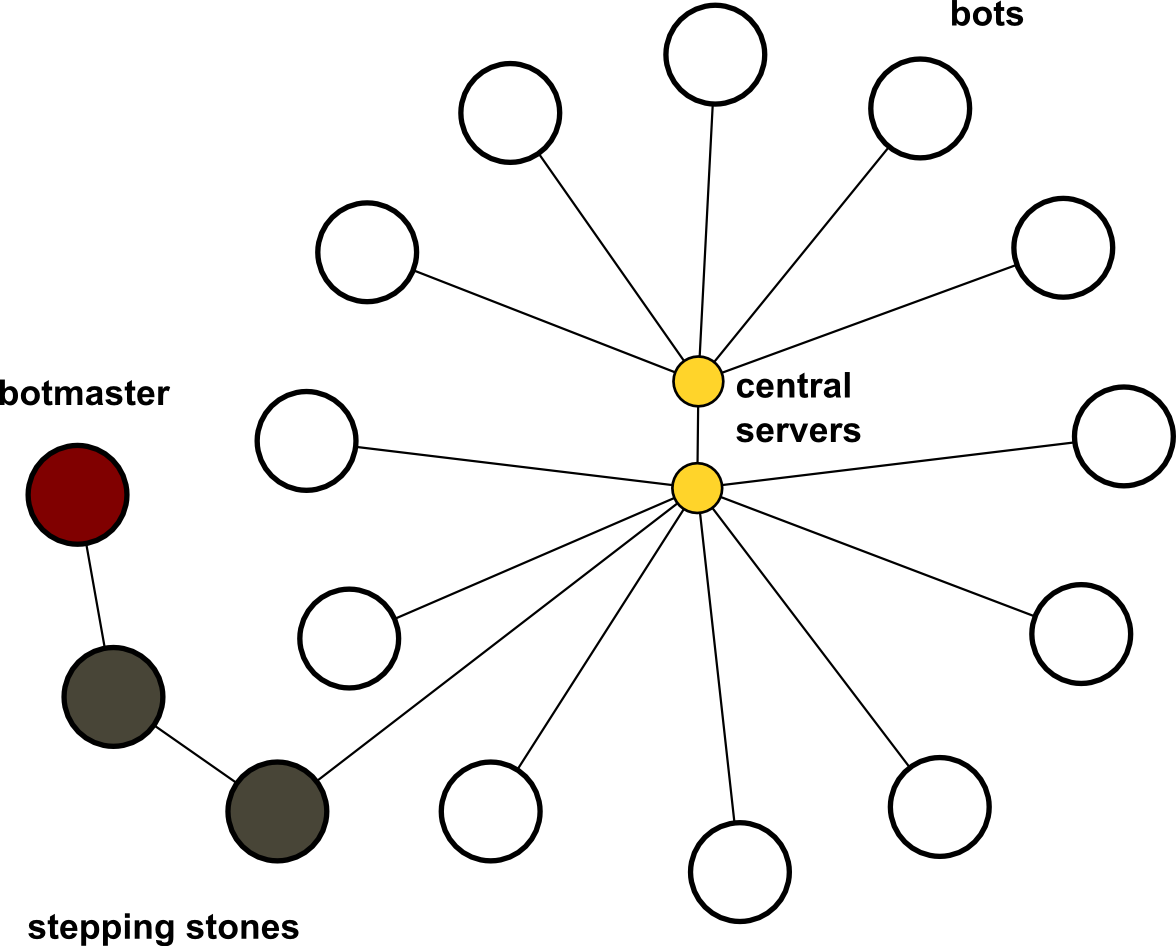
\includegraphics[width=0.8\textwidth]{figures/central-network.png}
  }
  \caption{Graph depicting connections in a centralised network. Note
    how all bots only have a connection to the central point. }
  \label{central-network}
\end{figure}
Historically the oldest form of botnets, centralised architectures are
built up in such a way that there is one central spot which broadcasts
messages between the connected bots and the botmaster.  It's common to
have more than one central server\cite{td1sc}, but even with several
servers, the architecture still stays centralised. For if you shutdown
this central point, the network is inoperable. This resembles the
biggest weakness of centralised architectures: As soon as you are able
to cut the server off the net, the network is dead. On the other hand,
latency becomes minimal, as the routing distance for one package
needed to reach each node in the botnet is minimal (only one
transition is needed). Bandwidth, however, is generally limited by the
server's resources, making it hard to receive or transmit big chunks
of data. Furthermore, it holds that all the routes in the botnet have
the same length. This is something which is fundamentally more complex
in decentralised networks and can be a great simplification of command
distribution and monitoring the network.

Due to their nature, centralised architectures are usually implemented
with an IRC C\&C or similar\cite{cooke2005zombie}. The central server
is normally not owned by the botmaster. This would make detecting his
identity easy. In many countries, launching an ``evil-minded botnet''
is a serious crime. Instead, hacked or public IRC servers are used as
the central C\&C node. A connection from the attacker's computer to
the central server is often obfuscated by many in-between relays,
tunnels and encryption. In figure
\ref{central-network} this is shown as the ``stepping stones'' which
shall hide an attacker's identity.

\subsection{Decentralised Architecture}
\label{decent}
Decentralised architectures do not rely on the special role of one
central server. Instead, they are built upon the principal of
equality, namely that the ``peer nodes (both client and server) are
all equal''\cite{steggink2007detection}. The topology of the network
is far more complex than in centralised architectures, forming a mesh
as shown in figure \ref{p2p-network}. It is thus more difficult for a
bot to join the botnet. Extensive bootstrapping is required, as the
bot has to figure out an already-participating peer to connect to in the
beginning. Once inside the net, information about other peers is
exchanged between nodes. There are two approaches for bootstrapping\cite{wang2009systematic}:
\begin{itemize}
\item A list of peers likely to be online is hard-coded into the client. This list can later be updated
\item A shared web cache on the internet stores information about
  peers. The address of which is hard-coded.
\end{itemize}

As can be seen, Bootstrapping is a critical and vulnerable point in
any P2P botnet. Considerable efforts by botmaster have been made to
circumvent the need to bootstrap\cite{td1sc}. This is further
discussed in section \ref{counter-measure}.

Once inside the net, information about other peers is
exchanged between nodes.

Distributing commands and data in such a network is complicated, as it
has to be assured that the message reaches all clients. As a general
rule of thumb, the better inter-connected the nodes are, the higher
the probability for a message to reach all recipients.

A decentralised network has the advantage of having the accumulated
resources and bandwidth of all the peers in the network
available. However, latency might be bad, as routing through the
network is not trivial (cf. figure \ref{p2p-network}). P2P networks
are generally considered to be harder to disable (cf. section
\ref{counter-measure} on page \pageref{counter-measure}). Another
advantage might be that the botmaster does not necessarily need to run
server of his own --- decreasing infrastructure costs in comparison
with centralised architectures.

\label{napsterlike}
It is to be discussed whether P2P networks with a centralised server
architecture for certain services like file-indexing --- we refer to
them as ``Napster-like'' botnets --- fall into the ``decentralised''
category. Principally, the connection graph differs a lot from
centralised networks, but centralised and Napster-like networks share
the same weaknesses, as could be seen when Napster was shut down in
2001\cite{napsterWiki}.\footnote{This was performed as an act of
  confirming with the decision made in the intellectual property case
  of US A\&M Records, Inc. v. Napster, Inc., 239 F.3d 1004 (2001) and
  not an explicit attack against the Napster network, but the fact
  that the Napster network could so easily stop the network by just
  disconnecting its central server shows the inherent weakness of
  centralised architectures.}  Dittrich et
al. \cite{dittrich2007command} would consider Napster-like botnets a
hybrid architecture, whereas Steggink et al.
\cite{steggink2007detection} classify it as decentralised. In the
following, we stick with Steggink's definition, as there seems to be a
broader consensus in the literature towards their nomenclature
(cf. \cite{td1sc}).

% P2P network picture
\begin{figure}[htbp]
  \centering
  \fbox{
    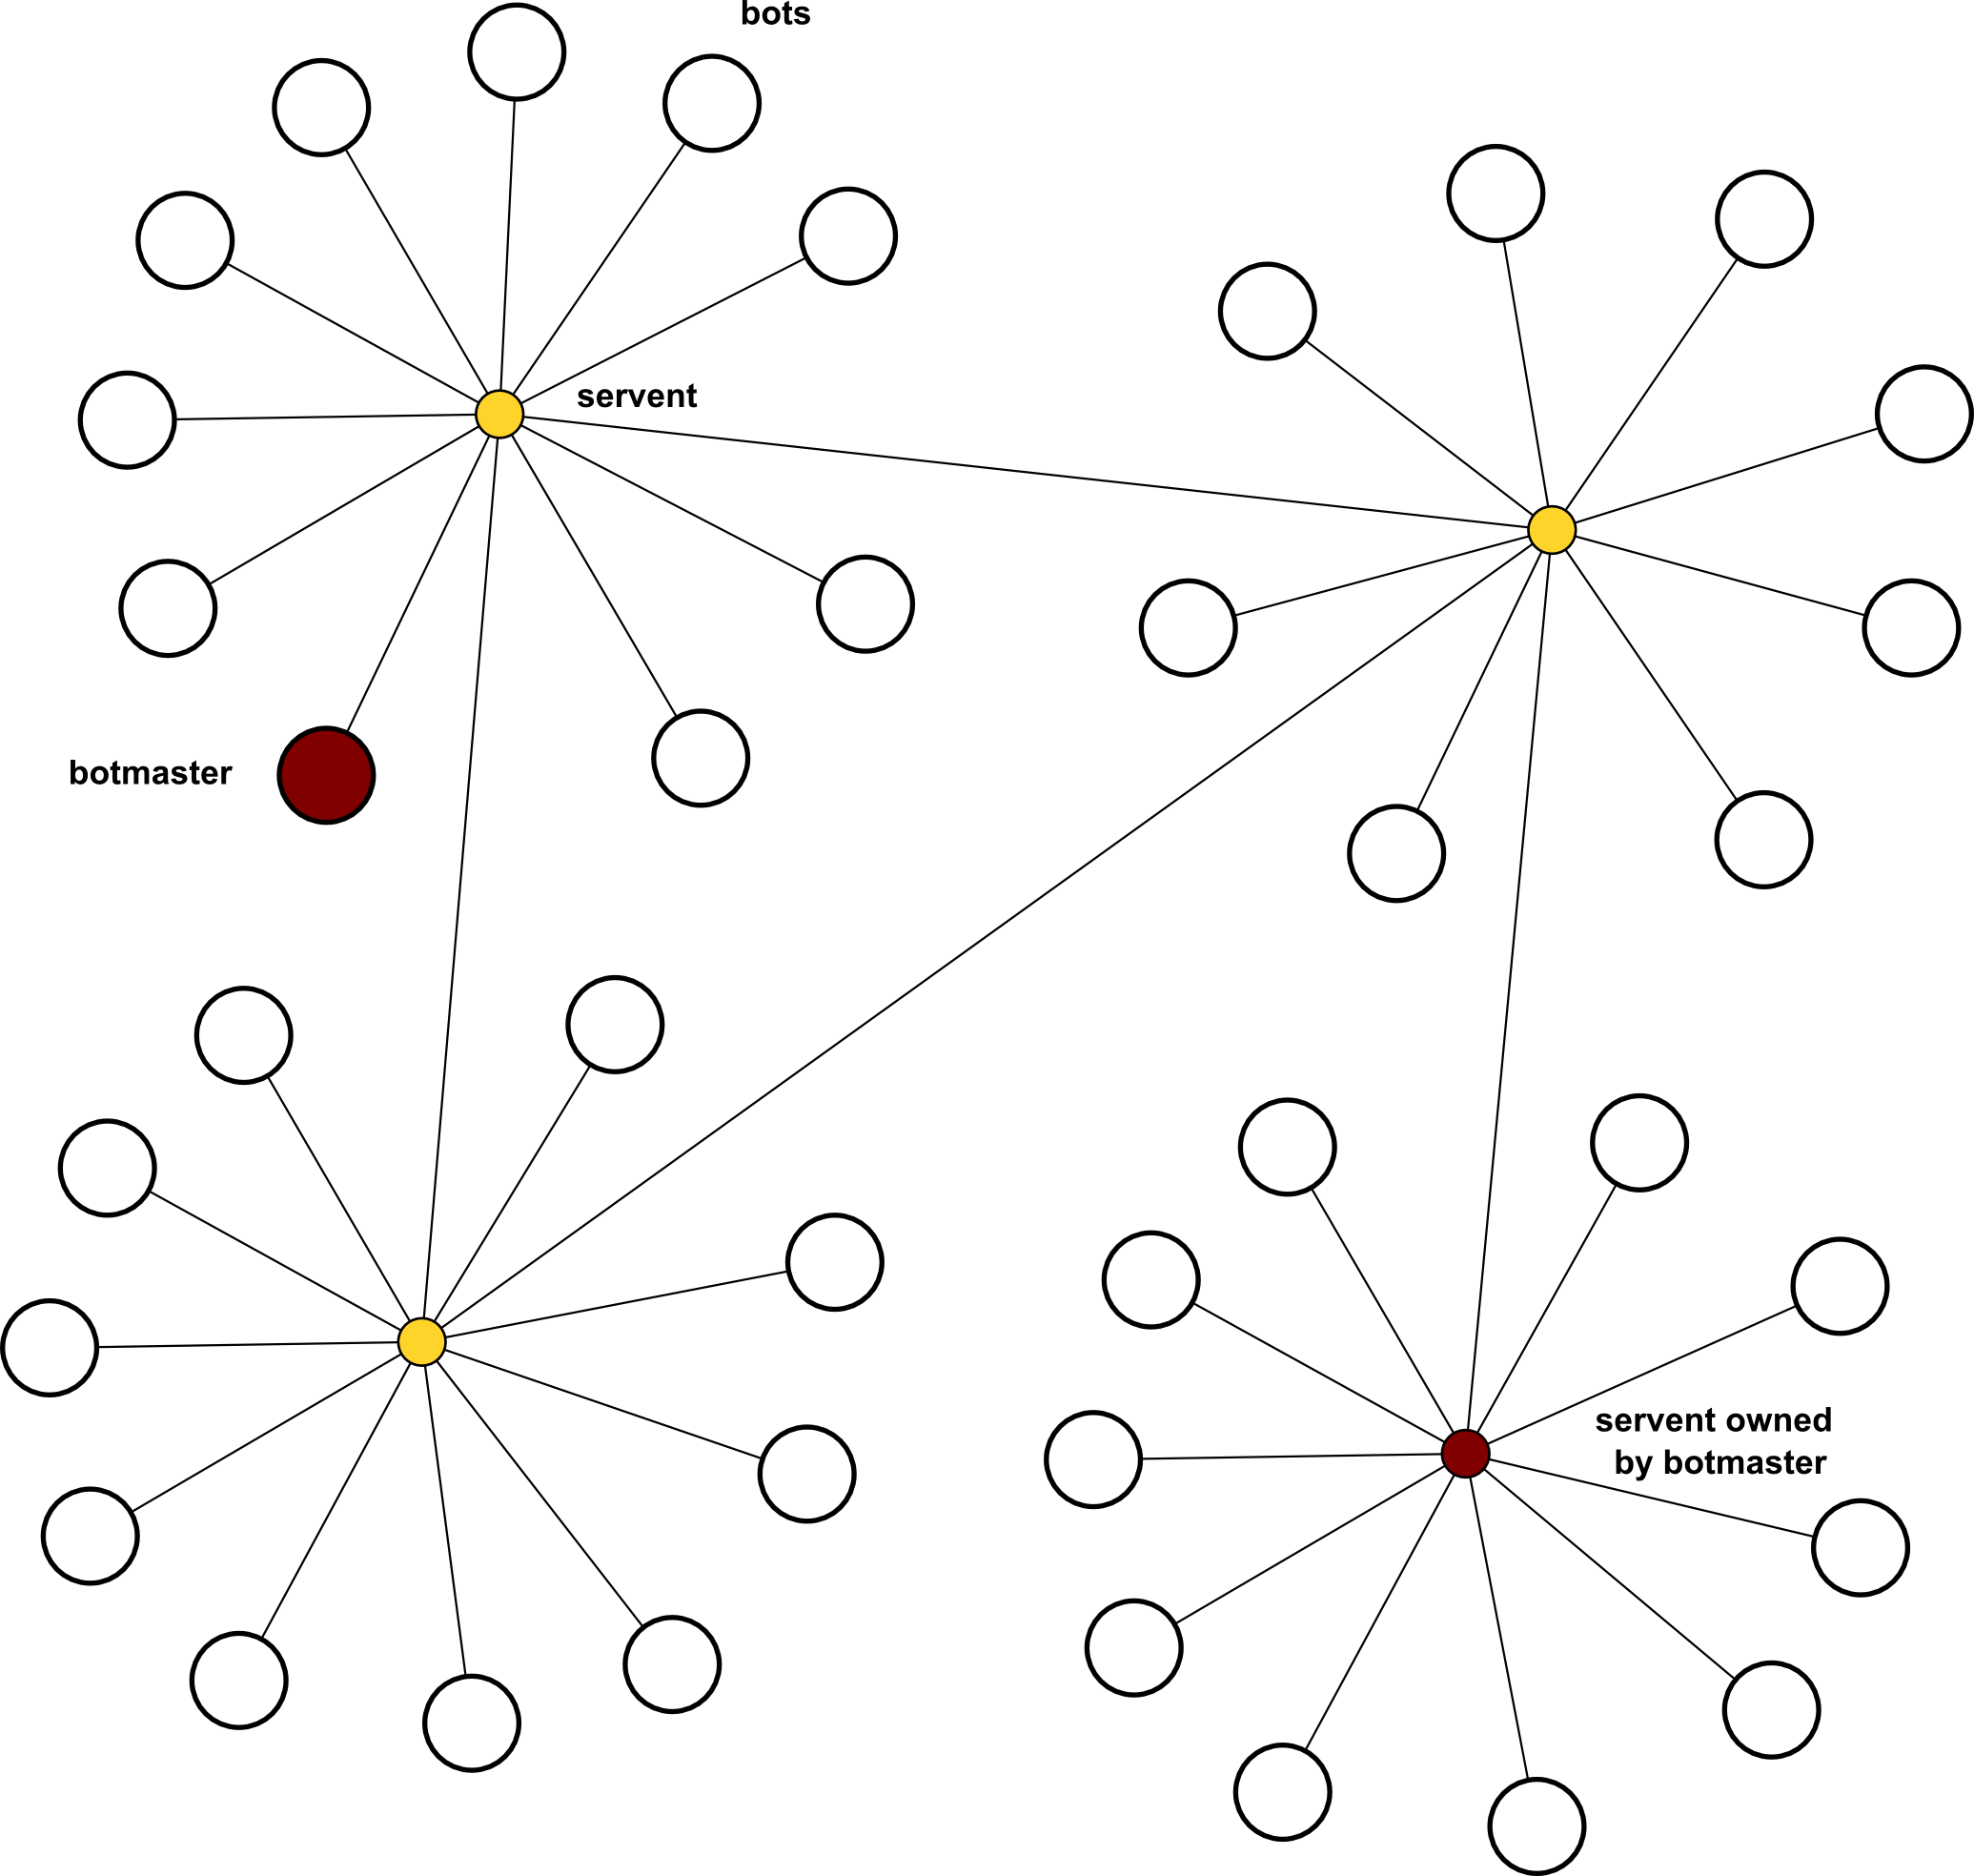
\includegraphics[width=0.9\textwidth]{figures/p2p-network.png}
  }
  \caption{An exemplary P2P network. The botmaster can be a regular
    peer, a servent/super peer/server (whatever the corresponding name
    in the underlying P2P network may be) or both. In contrast to other peers
    he injects new commands to be forwarded by others. It might make
    sense for the botmaster to own a few peers or servents, as this
    makes command distribution faster and increases his control over
    the network.}
  \label{p2p-network}
\end{figure}


\subsection{Hybrid Architecture}
\label{hybrid}
Hybrid architectures are botnet architectures driven by scientific
development and up to this date only exist in theory. They have been
described as ``the advanced P2P botnet''\cite{td1sc} and the ``super
botnet''\cite{vogt2007army}. The approach is to study current botnets,
analyse their weaknesses and propose a better solution. This
anticipates how botmasters could improve their botnets in the
future. This way, even today, we know what future botnets could look
like and how to better defend against them.

The proposed new hybrid P2P botnets do not have a pre-set
communication architecture, following the strict P2P definition. Their
network connectivity is solely determined by the {\it peer list} in
each bot.

Only machines with static IPs appear as bots in the peer list,
so-called {\it servents}. \cite{td1sc} This way, it is guaranteed that
the distributed peer lists are maximally deadlink-free.  This is a
specialisation of the ``all peers are equal'' contract in P2P: Some
bots --- the servents --- have special obligations described in the
following.  The clients are then typically bots behind firewalls,
machines with private or dynamic IPs.

\subsubsection{Network construction phase}

Infection is done no different than in conventional botnets
(cf. section \ref{ClassificP2P}). The basic construction procedure has two
mechanisms:
\begin{itemize}
\item {\bf New Infection:} ``Bot A passes its peer list to a
vulnerable host B when compromising it. If A is a
servent bot, B adds A into its peer list (by randomly
replacing one entry if its peer list is full). If A knows
that B is a servent bot (A may not be aware of
B’s identity, for example, when B is compromised by
an e-mail virus sent from A), A adds B into its peer
list in the same way.'' \cite{td1sc}
\item {\bf Reinfection:} ``If bot A
reinfects bot B, bot B will then replace \lbrack{}a series of\rbrack{} 
 randomly selected bots in its peer list with \lbrack{}...\rbrack{} bots
from the peer list provided by A. Again, bots A and B
will add each other into their respective peer lists if
the other one is a servent bot.''\cite{td1sc}
\end{itemize}

Both the advanced P2P botnet and the super botnet have their own P2P
protocols for C\&C. They implement push and pull
C\&C.\cite{wang2009systematic} When a bot receives a command it
forwards it to all the peers in its list (push). If a bot cannot
accept incoming connections (due to network misconfiguration, or a
firewall), it actively polls other peers in its connection list from
time to time to receive new commands (pull, cf. section \ref{pushpull}
on page \pageref{pushpull}).

\subsubsection{Lifetime Comparison against super botnet}

In the following, we will concentrate on the ``the advanced P2P
botnet'' as described by \cite{td1sc}. It was shown by Wang et
al. \cite{td1sc} that the super botnet suggested by Vogt et al. is not
likely to become successful in a real world scenario:

% distribution graph picture
\begin{figure}[htbp]
  \centering
  
    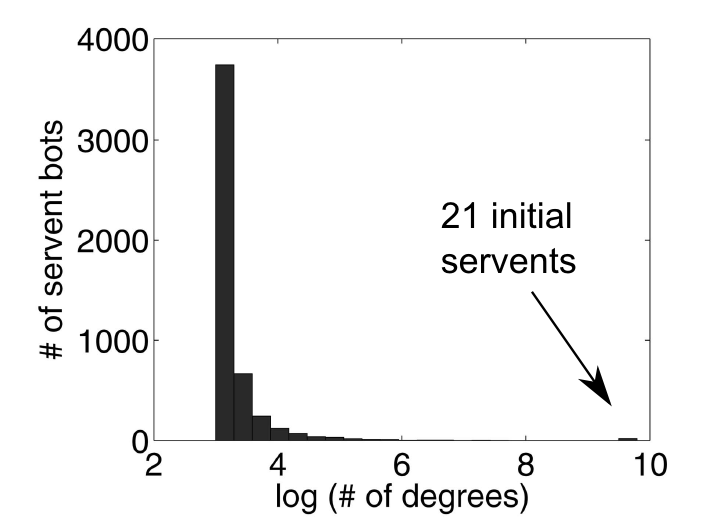
\includegraphics[width=0.6\textwidth]{figures/distributiongraph.png}
  
  \caption{Degree-distribution graph of servent bots assuming only new-infections and reinfections (derived work, original source: \cite{td1sc}). Simulation constraints: possible vulnerable hosts $n=500,000$, stop of growth of botnet after $n=20,000$, peer list size $M=20$, 21 initial servent bots.}
  \label{distributiongraph}
\end{figure}

% distribution graph picture
\begin{figure}[htbp]
  \centering
  
    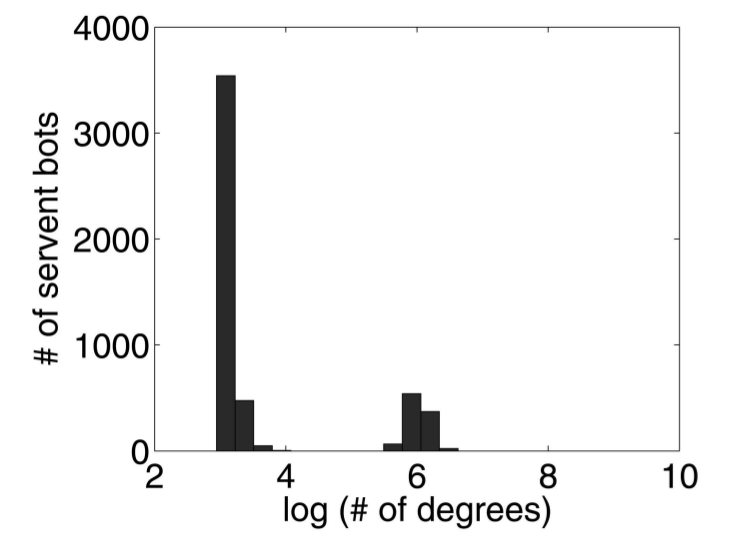
\includegraphics[width=0.6\textwidth]{figures/distributiongraph2.png}
  
  \caption{Degree-distribution graph of servent bots simulating peer list update propagation, also (Source: \cite{td1sc}). Most notably, the 21 initial servent bots cannot be spotted. Instead, a robust backbone for the P2P network has formed out of 1,000 servent bots $v$ (around x-axis 6), $deg(v) \in [300;500]$.}
  \label{distributiongraph2}
\end{figure}

\item \label{nat} In contrast to what Vogt et al. assume, most of the
  compromised computers cannot act as servents (due to a firewall,
  NAT\footnote{Network Address Translation, occurs behind a router}
  or dynamic IP address) in the real world.
\item Even though Vogt et al. demonstrated the robustness of their
  constructed botnet (cf. \cite{vogt2007army}), they rely on the
  assumption that enough reinfections will occur during the early
  lifetime of the botnet, namely the buildup-phase. According to
  \cite{td1sc} this is a false assumption as heavy reinfection-seeking
  during buildup will lead to easy detection of the botnet and a lot
  of wasted resources. Following this approach, Wang et al. showed
  that the super botnet algorithms for propagation --- namely only
  ``new infection'' and ``reinfection'' --- require over 200,000
  infections events to create an evenly balanced botnet of only 20,000
  vulnerable bots. As a result, when not enough reinfections occur, a
  scenario as depicted in figure \ref{distributiongraph} arises:
  Because the botnet stops growth after having infected 20,000 hosts,
  but there is such a huge amount of vulnerable hosts (500,000), a
  reinfection event rarely ever happens. This means that servent bots
  only seldom exchange parts of their peer lists. As a consequence,
  the connection to servent bots is extremely unbalanced: In the
  network graph, 80\% of servent bots have a degree\footnote{Degree is
    meant in the graph-theoretical sense here, i.e. counting the
    outgoing and incoming number of edges} less than 30, while the
  initial 21 servents have degrees between 14,000 -- 17,000: Most of
  the newly introduced servents have very few peers (both clients and
  servents) connected to them, essentially degrading the P2P botnet to
  a central network with 21 main servers. This is by no means an ideal
  P2P botnet.

When it is not possible to have enough reinfections, the ``new
infection'' and ``reinfection'' propagation measures are obviously not
enough.

\subsubsection{Peer list updating}
Because of this problem, Wang et al. propose a new, third propagation
method: Peer list updating. The idea behind this is that bots update
their peer lists frequently. However, this imposes a severe security
problem: An attacker capturing only one bot could soon reveal the
identity of many servents in the network. Thus, a new command is
introduced: Enforced peer list updating. As described in \cite{td1sc},
it is possible for a botmaster to monitor his botnet, i.e. determine
how many servents exist. After a sufficiently large time after
construction phase, he can enforce a peer list update: All bots obtain
a new peer list from a specified {\it sensor host}. This sensor host
is equipped with the knowledge of all the servents in the network by
the monitor-command issued by the botmaster. Upon query, the sensor
host creates a peer list in the following way: It randomly chooses
servent bots, composes an updated peer list out of them and sends it
back to the querying bot. After each peer list update command, all
bots will have ``uniform and balanced connections.''\cite{td1sc}

The network graph obtained is then similar to the one shown in figure
\ref{p2p-network} on page~\pageref{p2p-network}.

It is to be discussed at which point in time it makes sense for the
botmaster to enforce a peer list update, for every update command
bears the risk of discovery of parts of the network. This is further
discussed in \cite{td1sc}. Simulations with an update after the first
1,000 infections show that this update strategy will result in a
degree distribution depicted in figure \ref{distributiongraph2}: The
first 1,000 servents have many balanced connections ($deg(v) \in
[300;500]$), forming the robust backbone and connecting the hybrid P2P
network tightly together. However, the remaining 4,000 servents
(connected to the network after the update-command was run) have the
known symptom of having degrees between 20-30, a situation well-known
from the simulations of the super botnet (cf. figure
\ref{distributiongraph}). Thus, a forced peer list update from time to
time seems necessary to make for a good P2P infrastructure.

\begin{figure}[htbp]
  \centering
  \fbox{
    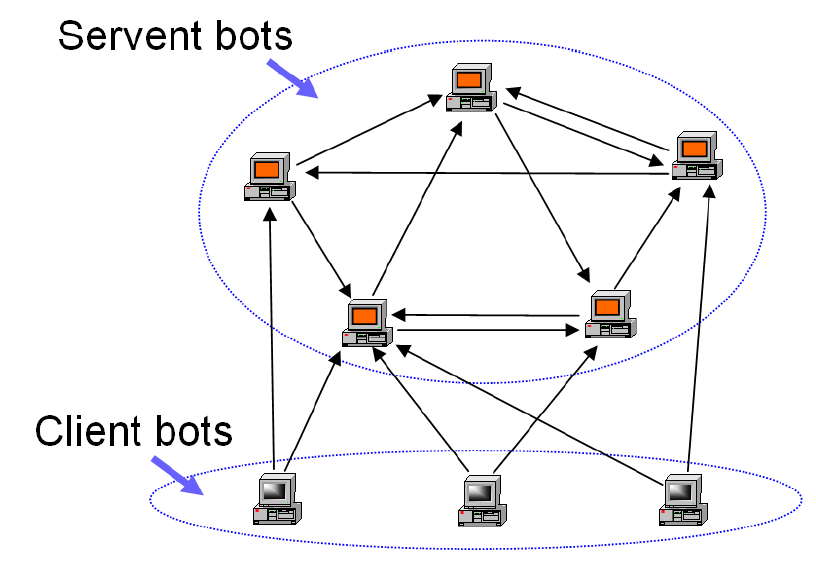
\includegraphics[width=0.7\textwidth]{figures/hybrid-network.png}
  }
  \caption{Hybrid network (Source: \cite{td1sc})}
  \label{hybrid-network}
\end{figure}

\subsubsection{Further improvements}
\label{hybridimprovs}
The proposed hybrid network has several other advantages over common,
existing P2P networks: It doesn't need bootstrapping, removing a
single point of failure. Bootstrapping is avoided due to the three
propagation measures (new infections, reinfections and forced peer
list updates). An initial peer list is simply passed on to the newly
infected zombie by the machine infecting it. Due to its fixed size
peer list ($M=20$ in the simulations for figures \ref{distributiongraph},
\ref{distributiongraph2}), when an attacker gets access to a bot, it
doesn't reveal whole (sub-)nets.  Only machines with static IPs appear
as peer bots, so-called {\it servents}. This way, it is guaranteed that
the distributed peer lists are maximally deadlink-free. Data
encryption in the hybrid P2P botnet has two functions: First, it makes
it hard to sniff for patterns in internet traffic to detect a possible
botnet. Second, the authenticity of the issued commands can be
verified so that only commands signed by the botmaster are
executed. The bot software can be shipped with a hard-coded public key
from the botmaster.

%% \begin{figure}[htbp]
%%   \centering
%%   \fbox{
%%     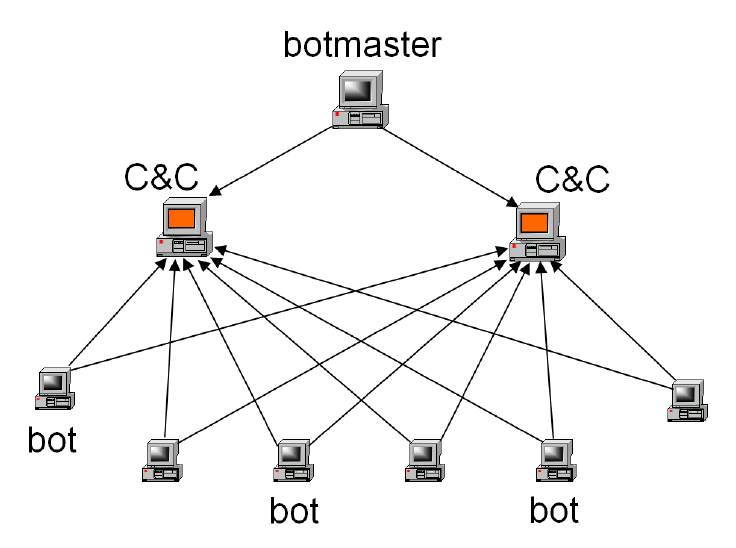
\includegraphics[width=0.7\textwidth]{figures/central-network2.png}
%%   }
%%   \caption{Another graphical representation of a central network (Source: \cite{td1sc})}
%%   \label{central-network2}
%% \end{figure}

Compared to a central-structure botnet (see figure
\ref{central-network}), the hybrid P2P net (see figure
\ref{hybrid-network}) is only an extension of the original network: It
is essentially equivalent to a central architecture P2P net. However,
the amount of servers (in the form of servents) is greatly increased,
as is the number of interconnections between them. The great number of
servents is the primary reason why the hybrid P2P botnet is supposedly
very hard to shut down.\cite{td1sc}

As tempting as such an advanced new botnet protocol may sound, it has
to be acknowledged that the hybrid P2P botnet is a purely academical,
theoretical idea that has never been tested in practice: ``The network
may not be as stable and robust as expected due to complex network
conditions and defences.''\cite{wang2009systematic}


\section{Countermeasures against evil P2P botnets}
\label{counter-measure}
What can an attacker do to de-arm a botnet at all? The ideal solution
would be to shutdown all participants in the botnet (and only
those). Realistically, this is almost never possible. It is also
illegal in most countries to start a botnet, as it implies gaining
access to another computer. This falls into the category of
hacking. On the other hand, paradoxically, shutting down a botnet is
likewise illegal, for it normally requires the attacker --- be he
benign or not --- to do the same: Hacking into computers. 

Common sub-tasks in fighting botnets are therefore, from an attacker's
perspective:

\begin{description}
\item {\bf Detecting the botnet} at all, which can be very difficult for P2P
  parasite and leeching networks, as a separation between ``bot'' P2P
  and ``real'' P2P data streams has to be made. For example, in
  \cite{steggink2007detection} it was shown that the bot Storm
  (therein referred to as ``Peacomm'') uses a fixed package size for
  95,4\% of its communication: 67 bytes (72,1\% of traffic) and 60 bytes
  (23,3\%). If one finds this atypical package size profile in a P2P
  network, it's likely to be infected by Storm.
\item {\bf Analysing the botnet:} Finding the servers (if there are any) and
  participating zombies. It is also helpful to be able to estimate the
  size of the botnet. When using a technique like sybil attacks (see
  section \ref{sybilattack}), this gives an estimation of how many resources
  are needed, i.e. how much money will be needed to take down the
  botnet.
\item {\bf Preventing further spread} of the botnet: Fixing the security
  exploit of the bot's injection vector. Most often, when a bot
  installs itself unnoticed from the owner ({\it injection}), it does so by
  using ({\it exploiting}) a security problem in the software. If the
  manufacturer fixes and updates this security hole, spread of the bot
  cannot continue on upgraded systems.
\item {\bf Disabling the bot(sub-)nets:} Making clients loose
  inter-connection (in P2P networks), shutting down central servers
  (in central networks).
\item {\bf Infiltrating botnets} to do non-malicious tasks, i.e. not to
  forward and not to execute incoming commands.
\end{description}

It must be noted that these tasks are of generic nature and might not
be applicable to the botnet at hand. However, they represent a solid
way of taking down a botnet.

While it is --- in theory --- relatively easy to shutdown a
centralised architecture by determining the central servers and
disabling those (e.g. through DoS attacks), P2P networks are arguably
harder to disable, given they are properly protected. The legal
implications of shutting down a botnet are also to be considered: When
proven to be malicious, it is possible for the police to get a warrant
to cut-off the servers physically from the net. This cannot
practically be done for non-centralised P2P networks, since the bots
are usually private property, with their owners unwillingly taking
part in the botnet. Additionally they usually exist in so great masses that a
physical take-down would be impossible to coordinate.

There are three well-known techniques to fight P2P botnets in
particular.

\subsection{Index poisoning}
\label{indexpoisoning}
\subsubsection{An attacker's idea: Polluting the file index}
The principal idea of index-poisoning is given by
\cite{wang2009systematic}: ``Originally, [the] index poisoning attack was
introduced to prevent illegal distribution of copyrighted content in
P2P networks. The main idea is to insert [a] massive number of bogus
records into the index. If a peer receives [a] bogus record, it could end
up not being able to locate the file (nonexistent location), or
downloading the wrong file.''

It is easy to transfer this idea to the C\&C of botnets. You only have
to think that bots are not usually looking for files, but for
commands. Once you know under which keys the botnet commands are
stored in the index records, an attacker trying to shutdown the
network can insert false commands under the same keys. If there is
enough false information, chances to hit the real command issued by
the botmaster are slim. The index gets ``flooded'' or poisoned by wrong
commands. These can either be NOPs (no operations, meaning a command
that does nothing), or may even help to uncover the botnet. Because
of its principal of inserting faulty records into a system, index
poisoning is also referred to as a ``pollution
attack''\cite{liang2006index}.

Index-poising has been reported to have succeeded
in fighting two recent P2P bots, namely Trojan.Peacomm and
Storm. (\cite{grizzard2007peer}, \cite{liang2006index})


\subsubsection{A botmaster's counter-defence: Authentication of commands}
It is an inherent property of any P2P network that any peer can and
should distribute commands. However, how can one achieve that only the
botmaster's commands are distributed and executed? In a centralised
architecture, this is relatively easy to assure: Only the botmaster
has the password to the servers, so only he can log onto them and
issue new commands. However, with P2P networks an encryption mechanism
for the commands must be implemented, such as public-key encryption (a
freely available example implementation is \cite{GPG}). The botmaster
signs (and possibly even encrypts) his commands with his private
key. By supplying the bot clients with the botmaster's public key,
they can authenticate the issuer of the command in question. As it is
very difficult to calculate the private key based on the public key,
bots can be assured that the issuer of the command is their
botmaster. For this to practically work, file index records $<k, m>$ ,
see section \ref{distribution}) could be enriched with a new column $H(m)$,
where $H(m)$ is the signed hash value of $m$, i.e. the signature of the
command.\cite{wang2009systematic} To verify $m$ has been issued by the
botmaster, a bot takes $H(m)$ and checks if it has been properly
signed by using the hard-coded public signature.


\subsection{Sybil attack}
\label{sybilattack}
\subsubsection{An attacker's idea: Inserting fake nodes}
A {\it sybil attack} on a botnet is a form of attack where large
quantities of fake nodes (the so-called sybils) are inserted into
the botnet. By infiltrating the botnet's peer list, the sybils try to
interrupt the C\&C between real bots. In contrast to the more static
pollution attack, a sybil attack requires the attacker to have active
hardware acting as the sybils and also to take part in the P2P
network. Note however, that it is not necessary and even
contra-indicative for the sybils to execute or distribute the commands
sent over the P2P network's C\&C structures. The idea of the sybil
attack lies in the fact that there exist so many sybils in the network
that issued commands get neither distributed nor executed. \cite{davis2008sybil}

Generally speaking, it is more expensive to run a sybil attack than an
index-poisoning attack, as the former requires far more infrastructure
at the disposal of the attacker.

\subsubsection{A botmaster's counter-defence}
Botmasters could utilise known P2P techniques to fight  the
weakness against sybil attacks: According to \cite{douceur2002sybil}, it is
common practice for a P2P system to distribute computational or
storage tasks among remote peers to protect against the threat of
hostile peers. For if a complete task is given to a hostile peer only,
chances are the task is never executed and completely lost. However,
this risk is mitigated when the task is replicated to several peers,
as it is unlikely for all peers to be hostile. In this way, a botnet
could at least slightly compensate for an ever-growing mass of sybils
in that its commands get executed anyway with a high probability
(determined by the level of redundancy introduced).

This does not solve the problem of sybils interrupting communication
in the first place. Countermeasures against this have been presented in
section \ref{hybrid} on page \pageref{hybrid}.

Sybil attacks have been simulated to be a valid countermeasure against
the Storm botnet.\cite{davis2008sybil}

\subsection{Compromising Bootstrapping}
Bootstrapping is a vulnerable point in any P2P botnet. When a
hard-coded peer list is used (cf. section \ref{decent} for details),
it is sufficient to take down all the peers in the bootstrapping table
for the network to eventually shutdown: New bots simply can't find an
initial peer to connect to. Botmasters have reacted to this by
providing a Gnutella-like web-cache or updateable bootstrapping
tables. As interrupting the bootstrapping process can so easily be
done, it has been completely removed in the hybrid botnets
(cf. section \ref{hybridimprovs} on page \pageref{hybridimprovs}).

\section{Conclusions and Outlook}
This paper gave an overview of the state-of-the-art in P2P
botnets. While \cite{wang2009systematic} conclude that a shutdown of a
P2P botnet is principally no harder than that of a central network
when employing the index poisoning technique, our understanding and
findings, as shown in this paper, are substantially different and
backed-up by both reason and literature (\cite{zou2006honeypot},
\cite{berger2009exploiting},
\cite{steggink2007detection}). Additionally, new P2P protocols can be
made resistant to index poisoning (shown in the same paper,
\cite{wang2009systematic}), or file indices can be completely omitted,
whereas the central nature of the servers remains a single point of
failure in centralised architectures.

In fact, because they are harder to disable, more agile and dynamic in
their life time, we believe that P2P botnets will play an ever-growing
role in the future. It can also be cheaper to setup a P2P botnet,
since there are no costs for central servers. Centralised
architectures on the other hand have been seen to decline and will
probably continue to do so. Also, some significant research for
improvement in the existing P2P protocols has been conducted,
removing many of the current weaknesses of P2P architectures.

\section*{Acknowledgement}
We would like to express our gratitude to Fabian Streitel for
reviewing this paper.

%------------------------------------------------------------------------------
\bibliographystyle{alpha}
\bibliography{literature}



\end{document}
